\subsubsection{Komponenter}
\paragraph{Motstand} \mbox{} \\
En motstand, også kalt resistor, er en komponent som begrenser strømmen.
Tenk på det som en kran du skrur igjen for å begrense antall elektroner som flyter forbi.
Det refererer også til et stoffs begrensede ledningsevne.
\\
Motstand noteres som $R$ (for resistance) og måles i ohm \SI{}{\ohm}.
\\
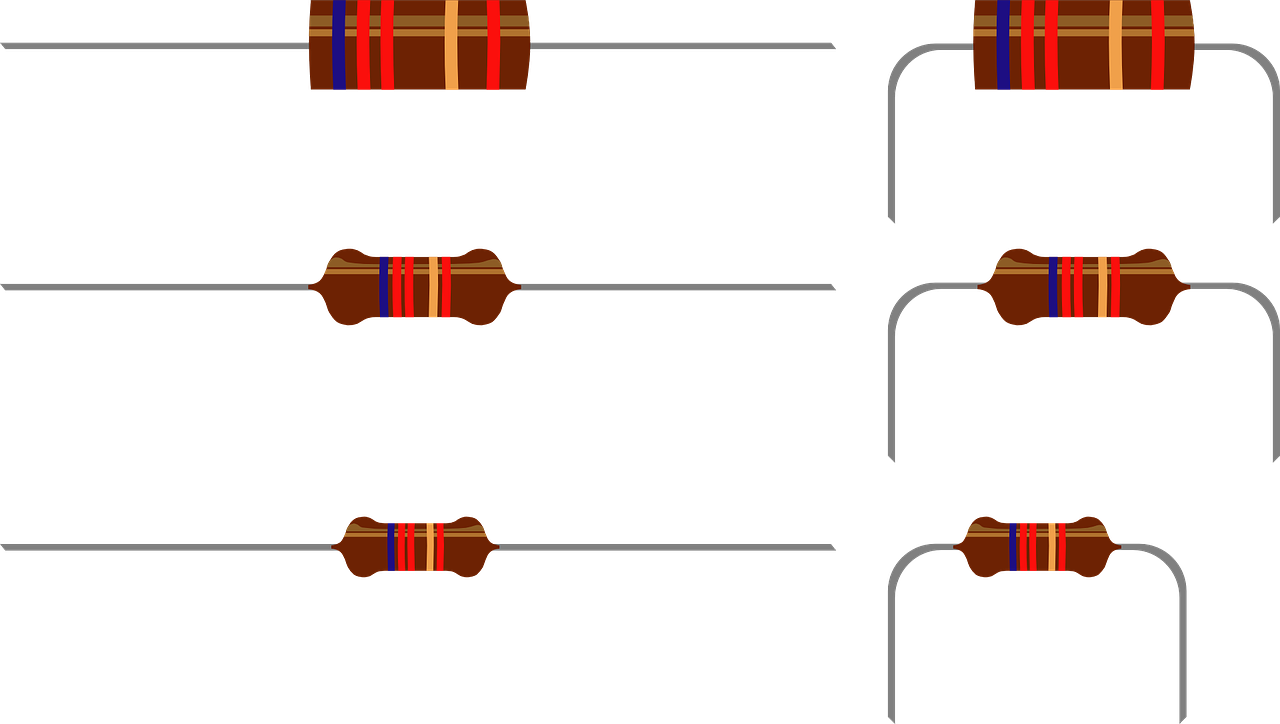
\includegraphics[width=0.33\textwidth]{./img/resistor}

\paragraph{Kondensator} \mbox{} \\
En kondensator (engelsk: capacitor) er litt som et batteri,
fordi den lagrer elektrisk energi.
\\
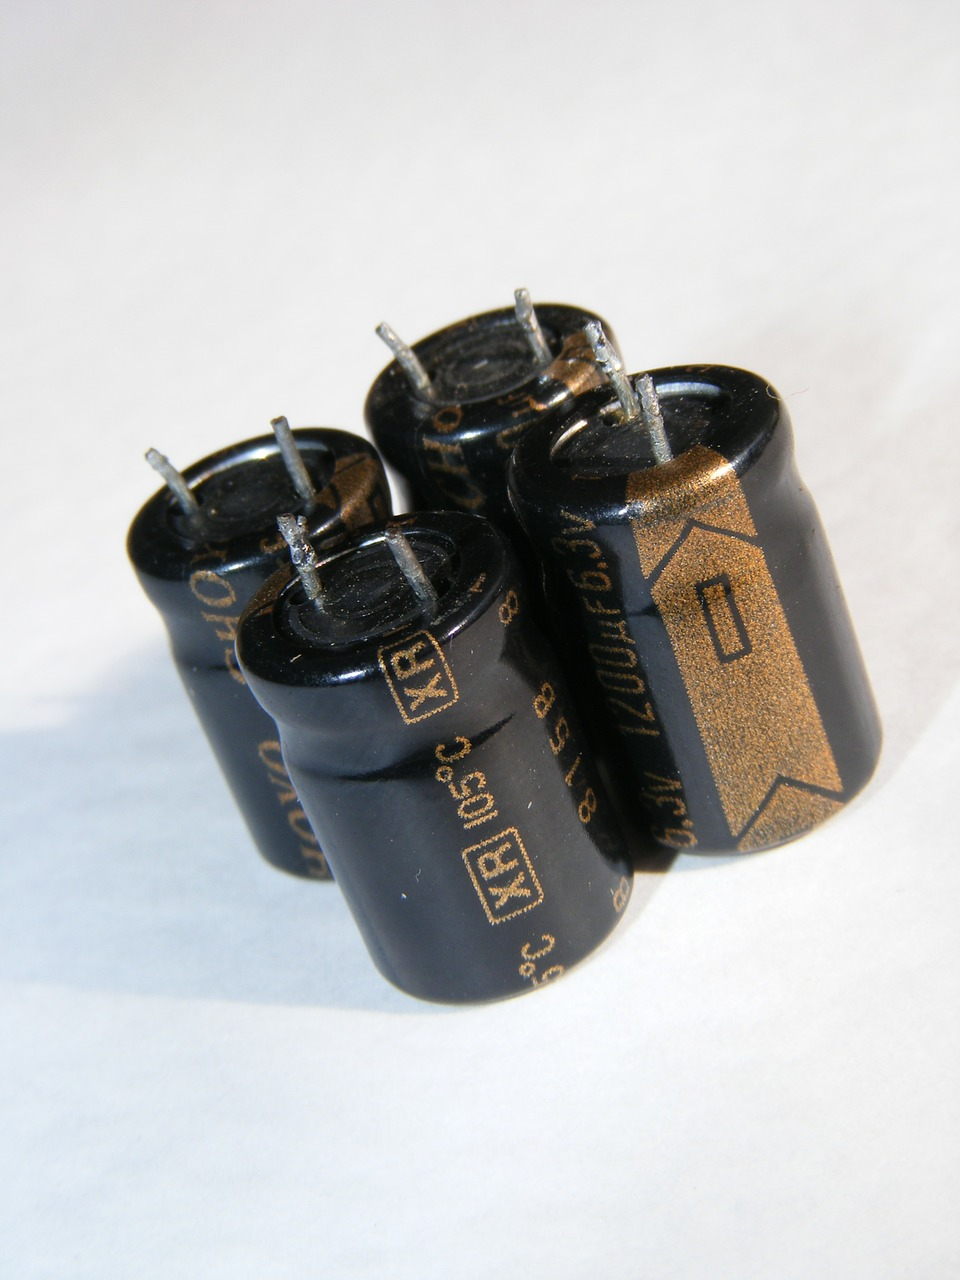
\includegraphics[width=0.33\textwidth]{./img/kondensator}

\paragraph{Spole} \mbox{} \\
En spole (engelsk: inductor) motstår forandring i strøm.
Det er likheter mellom funksjonen til en spole og en kondensator, men måten de fungerer på er forksjellig.
Mer om både kondensator og spole i senere kapitler.
